\documentclass{beamer}
    \usepackage[utf8]{inputenc}
    
    \usetheme{Madrid}
    \usecolortheme{default}
    \usepackage{amsmath,amssymb,amsfonts,amsthm}
    \usepackage{mathtools}
    \usepackage{txfonts}
    \usepackage{tkz-euclide}
    \usepackage{listings}
    \usepackage{adjustbox}
    \usepackage{array}
    \usepackage{gensymb}
    \usepackage{tabularx}
    \usepackage{gvv}
    \usepackage{lmodern}
    \usepackage{circuitikz}
    \usepackage{tikz}
    \lstset{literate={·}{{$\cdot$}}1 {λ}{{$\lambda$}}1 {→}{{$\to$}}1}
    \usepackage{graphicx}
    
    \setbeamertemplate{page number in head/foot}[totalframenumber]
    
    \usepackage{tcolorbox}
    \tcbuselibrary{minted,breakable,xparse,skins}
    
    
    
    \definecolor{bg}{gray}{0.95}
    \DeclareTCBListing{mintedbox}{O{}m!O{}}{%
      breakable=true,
      listing engine=minted,
      listing only,
      minted language=#2,
      minted style=default,
      minted options={%
        linenos,
        gobble=0,
        breaklines=true,
        breakafter=,,
        fontsize=\small,
        numbersep=8pt,
        #1},
      boxsep=0pt,
      left skip=0pt,
      right skip=0pt,
      left=25pt,
      right=0pt,
      top=3pt,
      bottom=3pt,
      arc=5pt,
      leftrule=0pt,
      rightrule=0pt,
      bottomrule=2pt,
      toprule=2pt,
      colback=bg,
      colframe=orange!70,
      enhanced,
      overlay={%
        \begin{tcbclipinterior}
        \fill[orange!20!white] (frame.south west) rectangle ([xshift=20pt]frame.north west);
        \end{tcbclipinterior}},
      #3,
    }
    \lstset{
        language=C,
        basicstyle=\ttfamily\small,
        keywordstyle=\color{blue},
        stringstyle=\color{orange},
        commentstyle=\color{green!60!black},
        numbers=left,
        numberstyle=\tiny\color{gray},
        breaklines=true,
        showstringspaces=false,
    }
    %------------------------------------------------------------
    %This block of code defines the information to appear in the
    %Title page
    \title %optional
    {12.561}
    \date{17 October, 2025}
    %\subtitle{A short story}
    
    \author % (optional)
    {INDHIRESH S - EE25BTECH11027}
    
    \begin{document}
    
    \frame{\titlepage}
    
    \begin{frame}{Question}
  The following system of equations
\begin{align*}
    2x-y-z=0\\
    -x+2y-z=0\\
    -x-y+2z=0
\end{align*}
\begin{enumerate}
    \item has no solution
    \item  has a unique solution
    \item  has three solutions.
    \item has an infinite number of solutions
\end{enumerate}
    \end{frame}
    
    \begin{frame}[allowframebreaks] 
    \frametitle{Equation}
        \centering
        \label{tab:parameters}
  The given eqaution can be given as:
\begin{align}
 \Vec{A}\Vec{x}=\Vec{B}
\end{align}


\begin{align}
  \myvec{2&-1&-1\\-1&2&-1\\-1&-1&2}\Vec{x}=\myvec{0\\0\\0}
\end{align}

    \end{frame}
    
    \begin{frame}
    \frametitle{Theoretical Solution}
   Now forming the augmented matrix and performing row operations
\begin{align}
   \augvec{3}{2}{2&-1&-1&0\\-1&2&-1&0\\-1&-1&2&0}\xleftrightarrow{R_1\longleftarrow R_2}\augvec{3}{2}{-1&2&-1&0\\2&-1&-1&0\\-1&-1&2&0}
\end{align}

\begin{align}
  \augvec{3}{2}{-1&2&-1&0\\2&-1&-1&0\\-1&-1&2&0}\xleftrightarrow{R_3\longleftarrow R_3-R_1}\augvec{3}{2}{-1&2&-1&0\\0&3&-3&0\\0&-3&3&0}
\end{align}

\begin{align}
\augvec{3}{2}{-1&2&-1&0\\0&3&-3&0\\0&-3&3&0}\xleftrightarrow{R_3\longleftarrow R_3+R_2}\augvec{3}{2}{-1&2&-1&0\\0&3&-3&0\\0&0&0&0}
\end{align}

Here the rank of the matrix is 2 which is less than 3.\\
So the system of the equation has an infinite number of solutions

    \end{frame}
    
    
    

    
    \begin{frame}{Plot}
        \begin{center}
            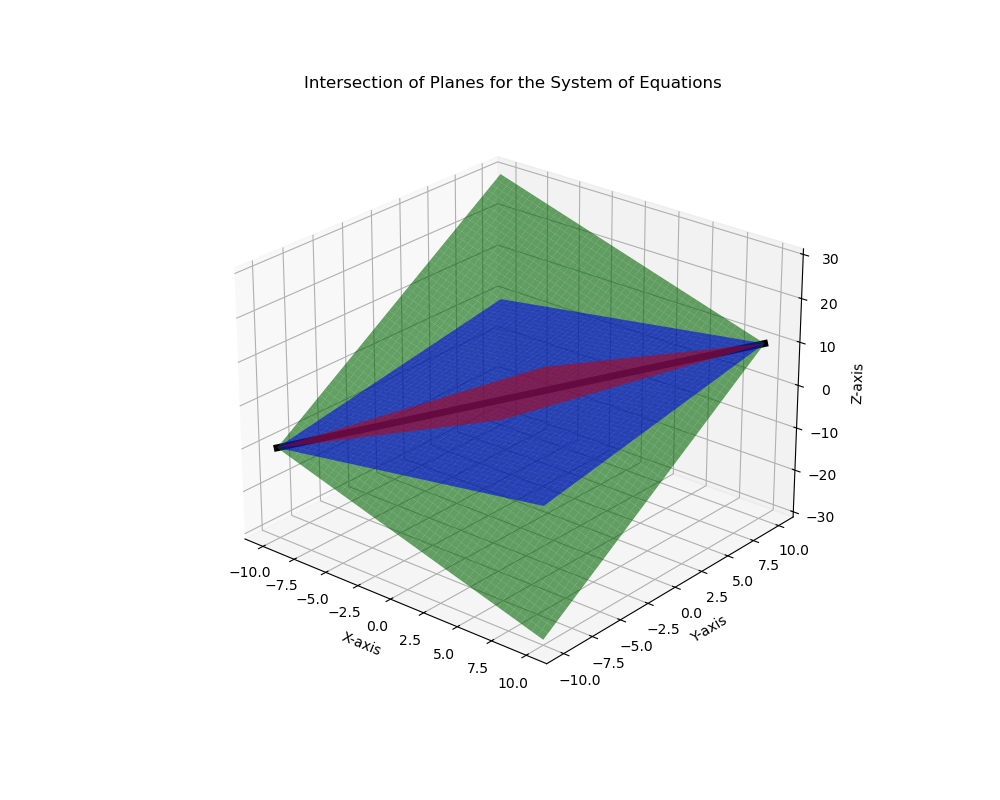
\includegraphics[width=\columnwidth, height=0.8\textheight, keepaspectratio]{figs/figure1.png}
        \end{center}
    \end{frame}
    
    \end{document}